\providecommand{\topdir}{..}
\documentclass[../main.tex]{subfiles}

\ifSubfilesClassLoaded{
  \externaldocument[main-]{../main}
  \externaldocument[fm-]{../00_front_matter/front_matter}
  \externaldocument[intro-]{../01_introduction/introduction}
  \externaldocument[l96-]{../02_lorenz96/lorenz96}
  \externaldocument[rb-]{../03_rayleigh_benard/rayleigh_benard}
  \externaldocument[tend-]{../04_tendencies/tendencies}
  \externaldocument[conc-]{../06_conclusion/conclusion}
  \externaldocument[app-]{../07_appendix/appendix}

  \setcounterref{chapter}{main-chap:evaluation}
  \addtocounter{chapter}{-1}
}{}

\begin{document}

\ifSubfilesClassLoaded{
    \frontmatter
    \tableofcontents
    \mainmatter
}{}

\dropchapter{0.5cm}
\chapter{Assessment of the parametrised model} \label{chap:evaluation}
\epigraphhead[0.1\textheight]{
    \epigraph{
        All models are wrong but some are useful.
    }{
        \emph{Robustness in the Strategy of\\Scientific Model Building} \\
        George Box, 1979
    }
}

In \cref{tend-chap:tendencies}, I analysed the subgrid tendencies and
constructed a statistical model \cref{tend-eqn:scheme_poly} to estimate
them from the coarse model tendencies. In this chapter, I will assess
the performance of the parametrised model obtained by coupling the
statistical model into the coarse \rb{} model.

First, a ``truth'' solution was obtained by running the fine (i.e., $2048
\times 256$; see \cref{tend-tab:final_resolutions}) model for 300 time units,
saving the output at intervals of 0.2 time units. The last snapshot from the
fine model simulation described in \cref{tend-sec:calculation}
(\cref{tend-itm:fine_model}) was used as the initial condition, thus keeping
the data used to test the parametrisation separate from the data used to fit
it. Every snapshot in the truth dataset was then coarse-grained using the
method described in \cref{tend-sec:coarse_graining}; the aim is for the
parametrised model to approximate this coarse-grained truth solution as closely
as possible.

A control solution was obtained by running the unmodified coarse (i.e., $256
\times 64$) model, using the first coarse-grained snapshot of the truth
solution as an initial condition. Output was saved at approximately the
same interval of 0.2 time units.

The equations governing the parametrised model, given schematically by
\cref{tend-eqn:res_tend_parametrised_model}, can be written out explicitly as
\begin{align*}
    \pdiff{\vec{u}}{t} &=
        \begin{pmatrix}
            1 + {\color{red} f_u(z)} & 0 \\
            0 & 1 + {\color{red} f_w(z)}
        \end{pmatrix}
        \left[
            -\vec{u} \cdot \grad \vec{u}
            -\grad \pi
            + \left( \frac{\prandtl}{\rayleigh}\right)^{1/2}
            \left(
                \nabla^2 \vec{u}
                + \tilde{\nu} f(z) |\nabla^2 \vec{u}| \nabla^2 \vec{u}
            \right)
            + \theta \uvec{z}
        \right], \\
    \pdiff{\theta}{t} &=
        (1 + {\color{red} f_\theta(z)}) \left[
            -\vec{u} \cdot \grad \theta
            + (\rayleigh\,\prandtl)^{-1/2}
            \left(
                \nabla^2 \theta
                + \tilde{\kappa} f(z) |\nabla^2 \theta| \nabla^2 \theta
            \right)
        \right], \quad \text{and} \\
    \grad \cdot \vec{u} &= 0,
\end{align*}
where the terms in red distinguish these modified equations from the originals
\crefrange{rb-eqn:hyper_momentum}{rb-eqn:hyper_incompressible}. The
parametrised model was run with the same resolution, time step, initial
condition and output interval as the control.

Unfortunately, when the parametrised model was run with the $f_\theta$,
$f_u$ and $f_w$ that were fitted in \cref{tend-sec:subgrid_modelling}, it
became unstable and crashed within 10 time units. Given the low coefficients
of determination for the $u$ and $w$ fits (\cref{tend-tab:r_squared}), I
chose to set $f_u(z) = f_w(z) \equiv 0$---that is, to only parametrise the
$\theta$ tendency and leave the momentum equation unmodified. This stabilised
the model.

\newpage
\section{Short-term forecast performance} \label{sec:forecast}

I first assess short-term accuracy using the root-mean-square error (RMSE)
of $u$, $w$ and $\theta$, defined by
\[
    \mathrm{RMSE}_\chi(t) = \sqrt{\langle
        (\chi_\mathrm{fc}(t) - \chi_\mathrm{truth}(t))^2
    \rangle _{x,z}},
\]
where $\chi = u, w, \theta$, $\chi_\mathrm{fc}$ is the forecast generated by
either the control or parametrised model and $\chi_\mathrm{truth}$ is the
\emph{coarse-grained} truth solution. \cref{fig:rmse} (a-c) compares the RMSE
of the control and parametrised solutions for the first 70 time units of
simulation.

Panel (a) shows that the $\theta$ RMSE of the parametrised model
initially grows at less than half the rate seen in the control, remaining
smaller than the control value for almost 10 time units before surpassing it.
While both models reach a peak RMSE before settling to a steady equilibrium,
the parametrised model takes approximately four times longer to do so. It seems
likely that by reducing the magnitude of $\partial\theta/\partial t$ near the
top and bottom of the domain, the parametrisation preserves the properties of
the thermal boundary layers. These are relatively thick and slowly-evolving in
the coarse-grained truth solution, but are thinned too quickly by the control
model.

For $u$ and $w$, the RMSE of the parametrised model initially increases
at a rate much closer to that of the control model. However, by plotting
the difference between the two and zooming the time axis (panels d-f),
it can be seen that the parametrised model does indeed have a slightly smaller
error.

\begin{figure}[ht]
    \centering
    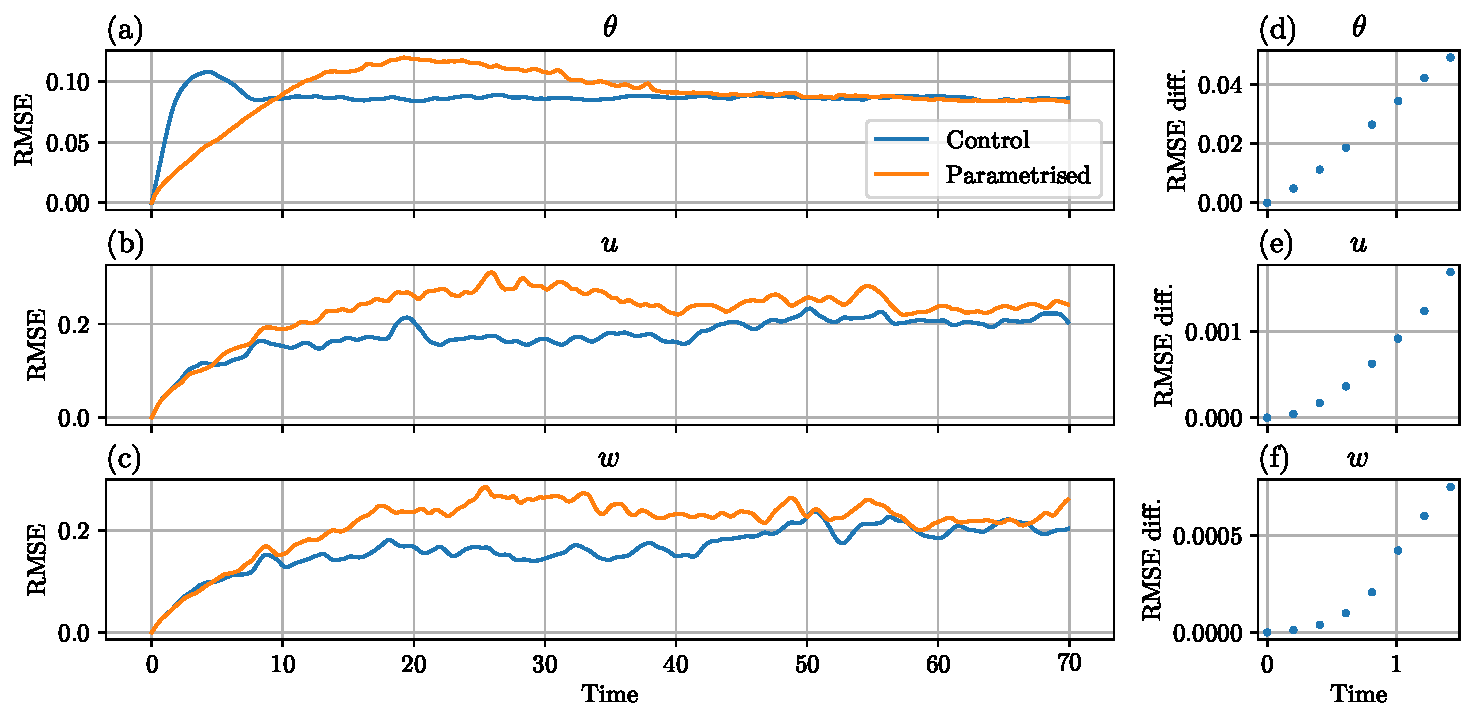
\includegraphics[width=\linewidth]{figures/rmse.pdf}
    \caption{
        \textbf{(a-c):} Root-mean-square error of the control (blue) and
        parametrised (orange) solutions for $\theta$, $u$ and $w$ over
        the first 70 time units of simulation. \textbf{(d-f):} The control
        RMSE minus the parametrised RMSE over the first 1.5 time units,
        confirming that the parametrised solution has lower RMSE in the short
        term.
    }
    \label{fig:rmse}
\end{figure}

Another way to assess short-term accuracy is to calculate domain-averaged
quantities for the parametrised, control and truth solutions and compare them
over time. As in \cref{rb-sec:choose_resolution}, I consider the Nusselt number
$\nusselt$, thermal boundary layer thickness $\delta_\theta$, RMS speed
$u_\mathrm{rms}$, kinetic energy dissipation rate $\epsilon_k$ and thermal
dissipation rate $\epsilon_\theta$, plotting their time series in
\cref{fig:short_term_metrics}. Both the control and parametrised models make
grossly inaccurate predictions for $\delta_\theta$ and $\epsilon_\theta$, but
the parametrised model's predictions are nonetheless closer to the truth for
the first $\sim 20$ time units. Since these are purely thermal quantities,
their improved prediction can be attributed to the nature of the
parametrisation scheme in the same way as the $\theta$ RMSE. The parametrised
model also makes more accurate initial predictions for the other three
quantities, but only for the first $\sim 5$ time units.

\begin{figure}[ht]
    \centering
    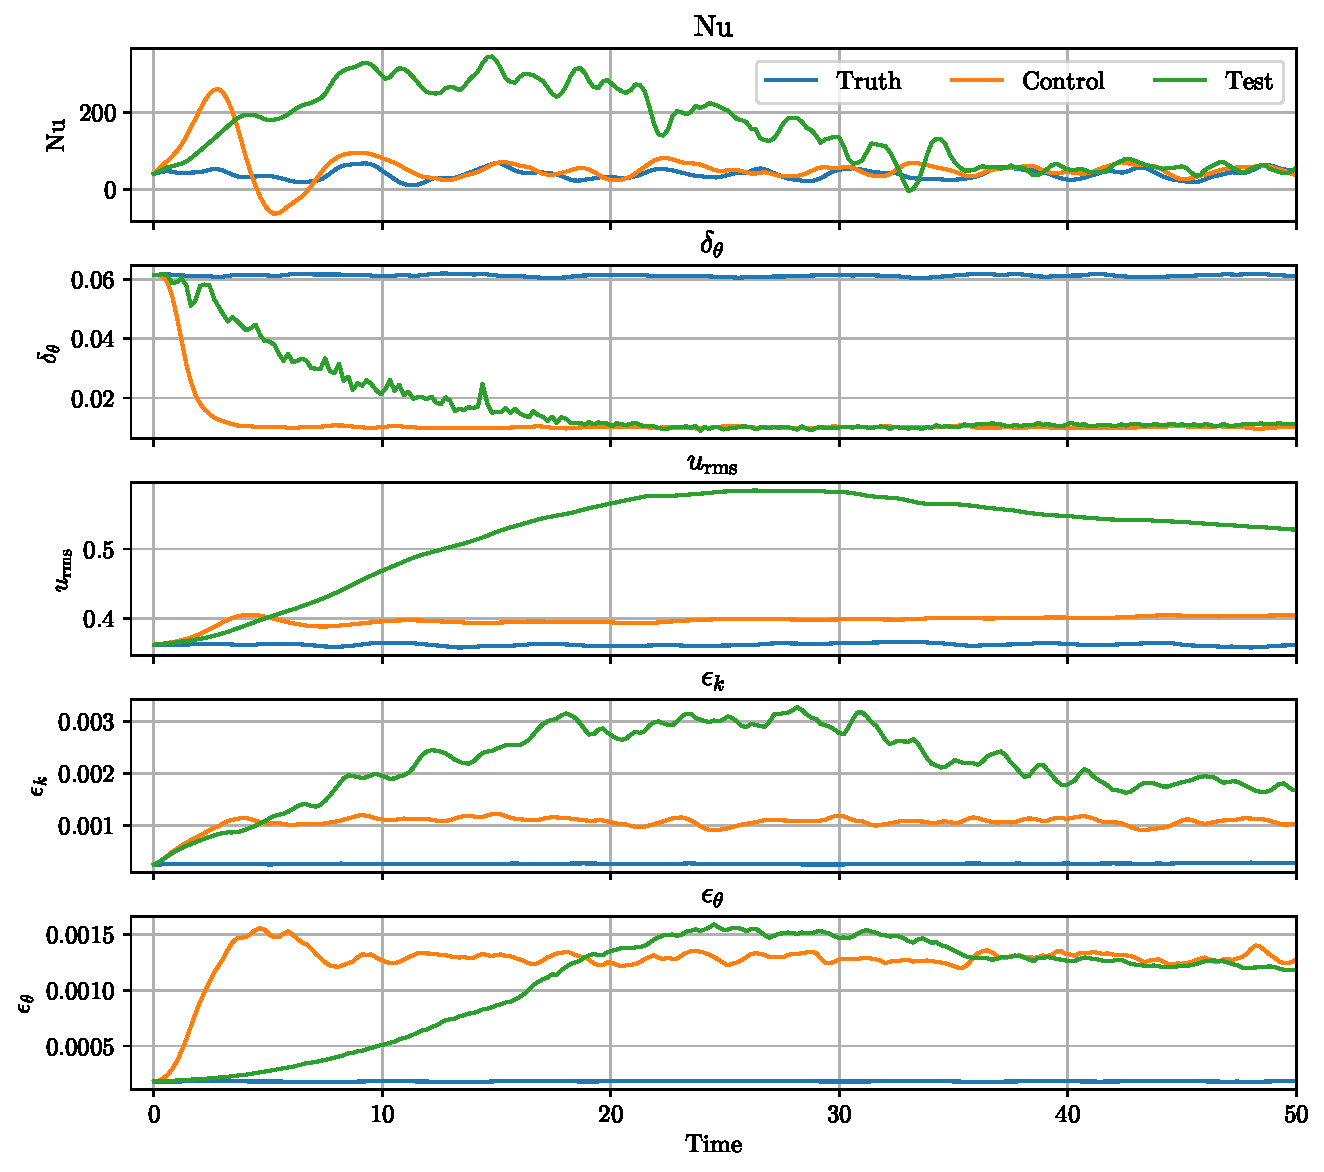
\includegraphics[width=\linewidth]{figures/short_term_metrics.pdf}
    \caption{
        Time series of the Nusselt number $\nusselt$, thermal boundary layer
        thickness $\delta_\theta$, RMS speed $u_\mathrm{rms}$, kinetic energy
        dissipation rate $\epsilon_k$ and thermal dissipation rate
        $\epsilon_\theta$ for the coarse-grained truth (blue), control (orange)
        and parametrised (green) solutions over the first 50 time units.
    }
    \label{fig:short_term_metrics}
\end{figure}

So far, I have shown that the parametrised model is capable of producing
more accurate short-term forecasts than the control if the lead time is
sufficiently short (on the order of a few time units)---a promising result.


\section{Accuracy of long-term statistics} \label{sec:climate}
\cref{sec:forecast} showed that, while the parametrised solution is more
accurate short-term forecasts, it is usually less accurate at longer lead
times. I now ask whether it will produce more accurate long-term statistics
if allowed to reach a statistically steady state.

The parametrised model was found
to take approximately 800 time units to return to a statistically steady state
(see \cref{app-sec:parametrised_spinup}). It was therefore integrated for
1100 time units, giving 300 time units of data for calculating long-term
statistics. For consistency, the control solution was also extended to 1100
time units.

\begin{figure}[ht]
    \centering
    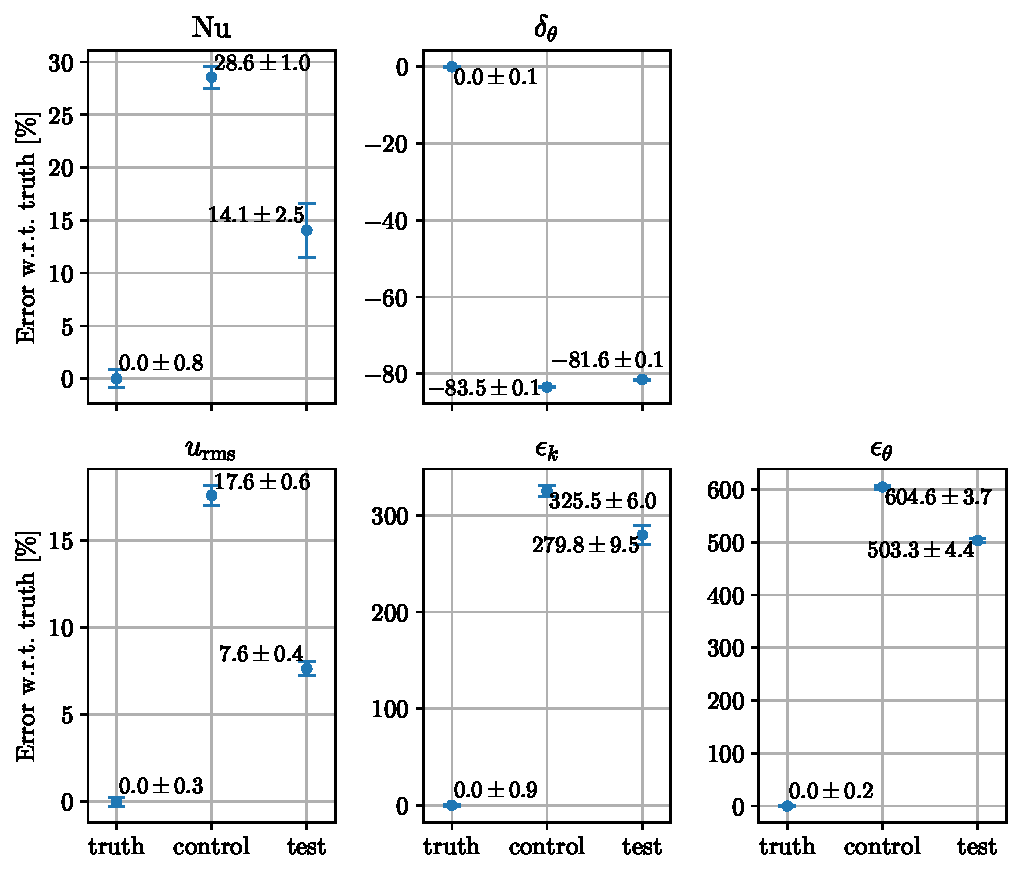
\includegraphics[width=0.65\linewidth]{figures/stats.pdf}
    \caption{
        F
    }
    \label{fig:stats}
\end{figure}

\begin{figure}[ht]
    \centering
    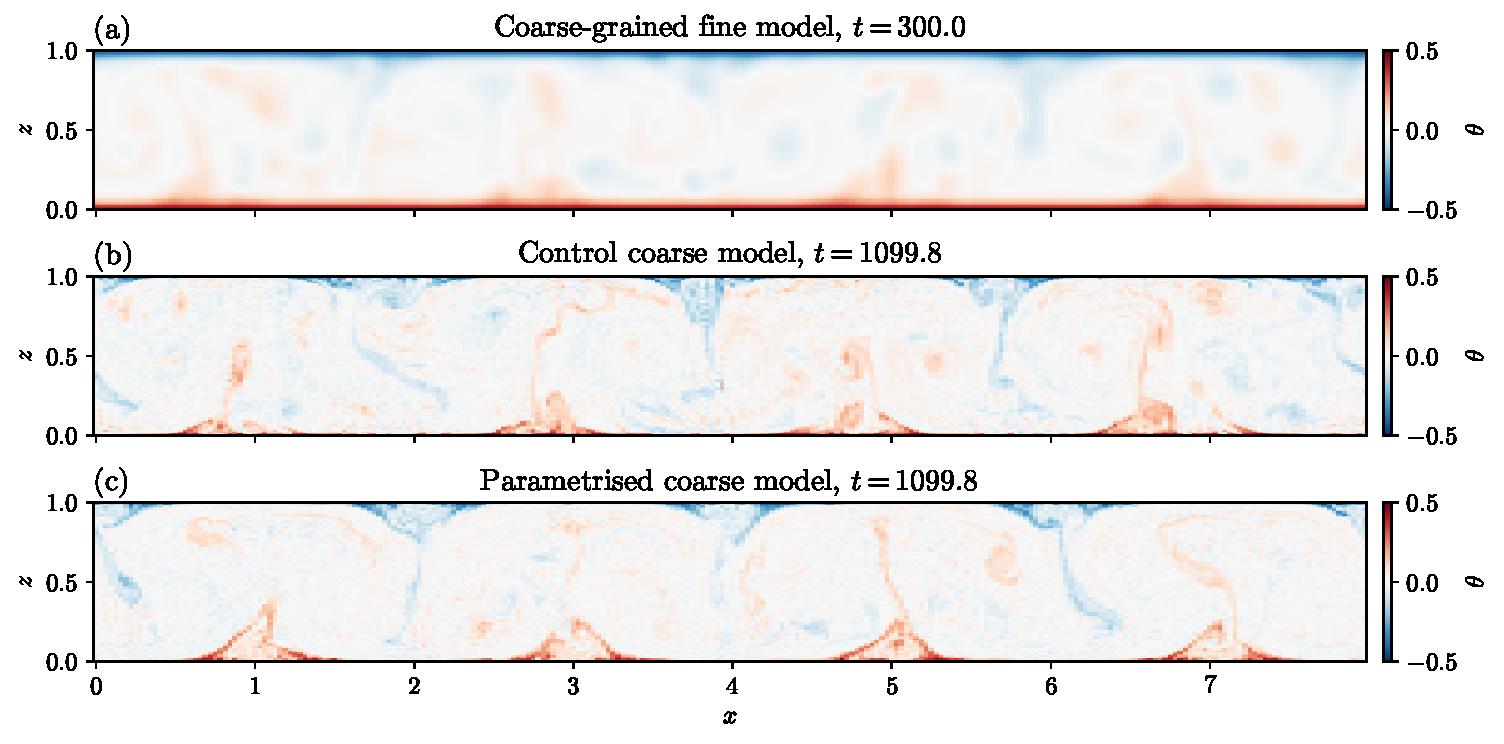
\includegraphics[width=\linewidth]{figures/steady_state_vis.pdf}
    \caption{
        F
    }
    \label{fig:steady_state_vis}
\end{figure}

\begin{figure}[ht]
    \centering
    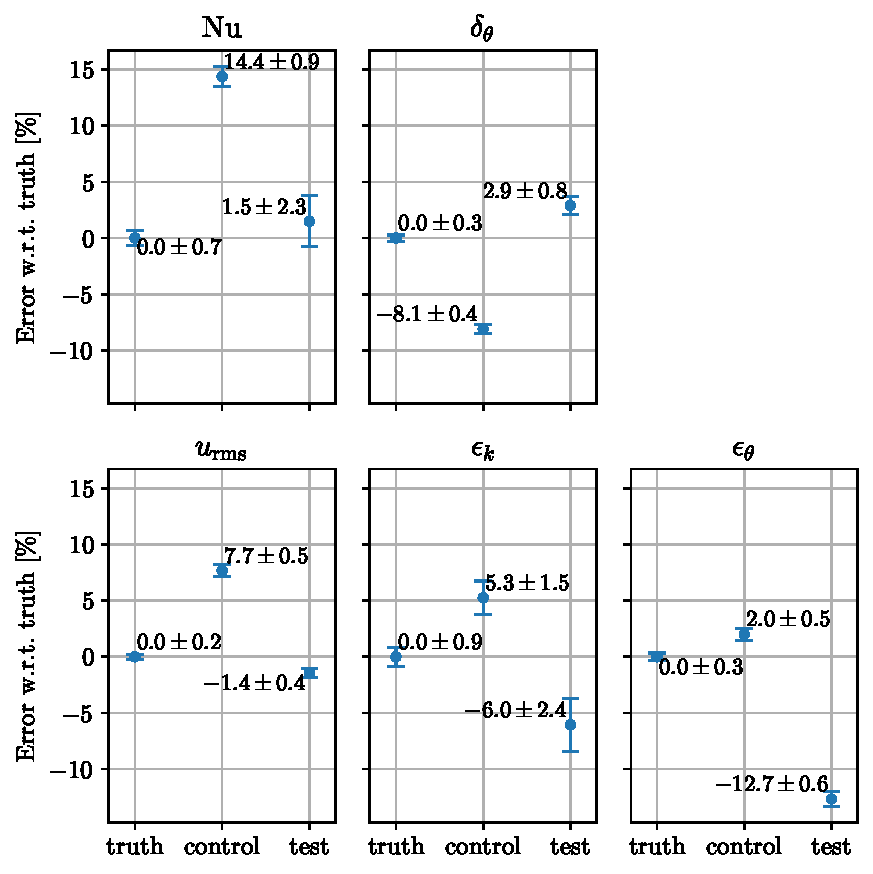
\includegraphics[width=0.65\linewidth]{figures/stats_vs_fine.pdf}
    \caption{
        F
    }
    \label{fig:stats_vs_fine}
\end{figure}

\ifSubfilesClassLoaded{%
    \emergencystretch=5em
    \printbibliography{}
}{}

\end{document}
